


\begin{figure}
  \setlength{\unitlength}{\textwidth}
  \begin{picture}(1,0.67)(0,0.35)
    
    % % %Parkinson Data 
    \put(0.025,0.95){\includegraphics[width=0.5\unitlength]{../FnP/gnuplot/displacement_amp_re_parkinson_1.eps}}
    \put(0.025,0.68){\includegraphics[width=0.5\unitlength]{../FnP/gnuplot/velocity_amp_re_parkinson.eps}}
    \put(0.025,0.41){\includegraphics[width=0.5\unitlength]{../FnP/gnuplot/mean_power_re_parkinson.eps}}
    
    % Re 165 Data 
    \put(0.495,0.95){\includegraphics[width=0.5\unitlength]{../FnP/gnuplot/displacement_amp_re165.eps}}
    \put(0.495,0.68){\includegraphics[width=0.5\unitlength]{../FnP/gnuplot/velocity_amp_re165.eps}}
    \put(0.495,0.41){\includegraphics[width=0.5\unitlength]{../FnP/gnuplot/mean_power_re_165.eps}}
      
    
       
   
%    \put(0.25,0.93){\ustar}
%    \put(0.8,0.93){\ustar}
%    \put(0.25,0.63){\ustar}
%   \put(0.8,0.63){\ustar}
    \put(0.25,0.39){\ustar}
     \put(0.75,0.39){\ustar}
    
    \put(0.00,1.075){$\frac{A}{D}$}
%    \put(0.52,1.075){$\frac{A}{D}$}
    \put(0.00,0.83){$\frac{V}{D}$}
%    \put(0.52,0.83){$\frac{V}{D}$}
    \put(-0.03,0.54){$\frac{P_{m}}{\rho \mathcal{A}U^3 }$}
%    \put(0.5,0.54){$\frac{P_{m}}{\rho \mathcal{A}U^3 }$}
    
    \put(0.06,0.95){(a) }
    \put(0.55,0.95){(b)}
    \put(0.06,0.68){(c)}
    \put(0.55,0.68){(d)}
    \put(0.06,0.41){(e)}
    \put(0.55,0.41){(f)}   
  \end{picture}
%  \vspace{-4cm}
  \caption{Velocity and displacement amplitude and mean power  as a function of $U^*$. (a), (c) and (e) are calculated using input $C_y$ data at Re=22300 obtained by \cite{Parkinson1964} and present data at three different damping ratios: $\zeta=0.0125$ (\ding{83}), $\zeta=0.015$ (\ding{116}) and $\zeta=0.0175$ (\ding{108}). (b),(d) and (f) are from $C_y$ data at Re=165 and are calculated  from the fixed body simulations and present data at three different  different damping ratios: $\zeta=0.075$ ($\times$), $\zeta=0.1$ (\ding{117}) and $\zeta=0.15$ (+). The multiple branches for the higher Re are due to the hysteresis between two solutions.}
  
  \label{fig:uncollapsed_data}
\end{figure}

